\begin{quote}
The path taken between two points by a ray of light\\is the path that can be traversed in the least time.\\- Pierre de Fermat
\end{quote}  

\begin{multicols}{2}
\section{Brechung}
\index{Optik!Brechung}
\begin{align*}
\frac{\sin{\varepsilon_1}}{\sin{\varepsilon_2}}&=\frac{n_2}{n_1}=\frac{c_1}{c_2}\\
\varepsilon_2&=\arcsin{\frac{\sin{\varepsilon_1}\cdot n_1}{n_2}}
\end{align*}

\section{Totalreflexion}
\index{Optik!Totalreflexion}
\begin{align*}
\sin{\varepsilon_g}&=\frac{n_2}{n_1}
\end{align*}

% Graphic for TeX using PGF
% Title: /home/befedo/Dokumente/eclipse.workspace/Formelsammlung/Physik/Brechung.dia
% Creator: Dia v0.97.2
% CreationDate: Wed Jul  4 16:39:00 2012
% For: befedo
% \usepackage{tikz}
% The following commands are not supported in PSTricks at present
% We define them conditionally, so when they are implemented,
% this pgf file will use them.
\ifx\du\undefined
  \newlength{\du}
\fi
\setlength{\du}{15\unitlength}
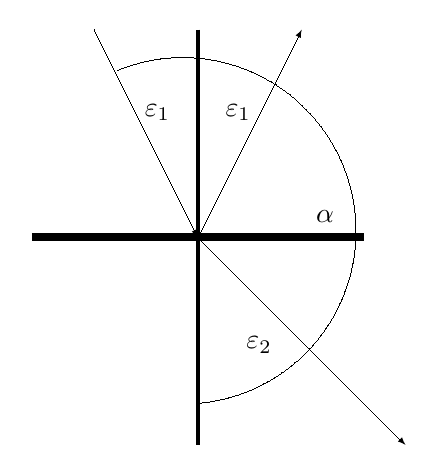
\begin{tikzpicture}
\pgftransformxscale{1.000000}
\pgftransformyscale{-1.000000}
\definecolor{dialinecolor}{rgb}{0.000000, 0.000000, 0.000000}
\pgfsetstrokecolor{dialinecolor}
\definecolor{dialinecolor}{rgb}{1.000000, 1.000000, 1.000000}
\pgfsetfillcolor{dialinecolor}
\pgfsetlinewidth{0.200000\du}
\pgfsetdash{}{0pt}
\pgfsetdash{}{0pt}
\pgfsetbuttcap
{
\definecolor{dialinecolor}{rgb}{0.000000, 0.000000, 0.000000}
\pgfsetfillcolor{dialinecolor}
% was here!!!
\definecolor{dialinecolor}{rgb}{0.000000, 0.000000, 0.000000}
\pgfsetstrokecolor{dialinecolor}
\draw (31.000000\du,5.000000\du)--(39.000000\du,5.000000\du);
}
\pgfsetlinewidth{0.100000\du}
\pgfsetdash{}{0pt}
\pgfsetdash{}{0pt}
\pgfsetbuttcap
{
\definecolor{dialinecolor}{rgb}{0.000000, 0.000000, 0.000000}
\pgfsetfillcolor{dialinecolor}
% was here!!!
\definecolor{dialinecolor}{rgb}{0.000000, 0.000000, 0.000000}
\pgfsetstrokecolor{dialinecolor}
\draw (35.000000\du,0.000000\du)--(35.000000\du,10.000000\du);
}
\pgfsetlinewidth{0.000000\du}
\pgfsetdash{}{0pt}
\pgfsetdash{}{0pt}
\pgfsetbuttcap
{
\definecolor{dialinecolor}{rgb}{0.000000, 0.000000, 0.000000}
\pgfsetfillcolor{dialinecolor}
% was here!!!
\pgfsetarrowsend{latex}
\definecolor{dialinecolor}{rgb}{0.000000, 0.000000, 0.000000}
\pgfsetstrokecolor{dialinecolor}
\draw (32.500000\du,0.000000\du)--(35.000000\du,5.000000\du);
}
\pgfsetlinewidth{0.000000\du}
\pgfsetdash{}{0pt}
\pgfsetdash{}{0pt}
\pgfsetbuttcap
{
\definecolor{dialinecolor}{rgb}{0.000000, 0.000000, 0.000000}
\pgfsetfillcolor{dialinecolor}
% was here!!!
\pgfsetarrowsend{latex}
\definecolor{dialinecolor}{rgb}{0.000000, 0.000000, 0.000000}
\pgfsetstrokecolor{dialinecolor}
\draw (35.000000\du,5.000000\du)--(37.500000\du,0.000000\du);
}
\pgfsetlinewidth{0.000000\du}
\pgfsetdash{}{0pt}
\pgfsetdash{}{0pt}
\pgfsetbuttcap
{
\definecolor{dialinecolor}{rgb}{0.000000, 0.000000, 0.000000}
\pgfsetfillcolor{dialinecolor}
% was here!!!
\pgfsetarrowsend{latex}
\definecolor{dialinecolor}{rgb}{0.000000, 0.000000, 0.000000}
\pgfsetstrokecolor{dialinecolor}
\draw (35.000000\du,5.000000\du)--(40.000000\du,10.000000\du);
}
\pgfsetlinewidth{0.000000\du}
\pgfsetdash{}{0pt}
\pgfsetdash{}{0pt}
\pgfsetbuttcap
{
\definecolor{dialinecolor}{rgb}{0.000000, 0.000000, 0.000000}
\pgfsetfillcolor{dialinecolor}
% was here!!!
\definecolor{dialinecolor}{rgb}{0.000000, 0.000000, 0.000000}
\pgfsetstrokecolor{dialinecolor}
\pgfpathmoveto{\pgfpoint{34.999665\du}{9.000030\du}}
\pgfpatharc{85}{-112}{4.172904\du and 4.172904\du}
\pgfusepath{stroke}
}
% setfont left to latex
\definecolor{dialinecolor}{rgb}{0.000000, 0.000000, 0.000000}
\pgfsetstrokecolor{dialinecolor}
\node[anchor=west] at (33.500000\du,2.000000\du){\(\varepsilon_1\)};
% setfont left to latex
\definecolor{dialinecolor}{rgb}{0.000000, 0.000000, 0.000000}
\pgfsetstrokecolor{dialinecolor}
\node[anchor=east] at (36.500000\du,2.000000\du){\(\varepsilon_1\)};
% setfont left to latex
\definecolor{dialinecolor}{rgb}{0.000000, 0.000000, 0.000000}
\pgfsetstrokecolor{dialinecolor}
\node[anchor=east] at (37.000000\du,7.595000\du){\(\varepsilon_2\)};
% setfont left to latex
\definecolor{dialinecolor}{rgb}{0.000000, 0.000000, 0.000000}
\pgfsetstrokecolor{dialinecolor}
\node[anchor=east] at (38.500000\du,4.500000\du){\(\alpha\)};
\end{tikzpicture}


Totalreflexion tritt nur auf, wenn der Lichtstrahl von einem dichteren in einen optisch
dünneren Stoff übergeht.

\end{multicols}

\section{Hohlspiegel}
\index{Optik!Hohlspiegel}
\begin{multicols}{2}
\begin{center}
 \includegraphics[width=60mm,keepaspectratio=true]{./Physik/Bilder/Hohlspiegel.png}
\end{center}

\begin{align*}
\frac{1}{f'}&=\frac{1}{a}+\frac{1}{a'}\\
f'&=\frac{r}{2}\\
\beta'&=\frac{y'}{y}\\
\beta'&=-\frac{a'}{a}
\end{align*}
\end{multicols}

\section{Linse}
\index{Optik!Linse}
\begin{multicols}{2}
\begin{center}
 \includegraphics[width=60mm,keepaspectratio=true]{./Physik/Bilder/Linse.png}
\end{center}
\begin{align*}
\frac{1}{f'}&=\frac{1}{a'}-\frac{1}{a}\\
\frac{1}{f}&=\frac{1}{a'}+\frac{1}{a}\\
f&=\frac{a\cdot a'}{a+a'}=-f'\\
a'&=\frac{af'}{a+f'}\\
\beta'&=\frac{f'}{a+f'}\\
\beta'&=\frac{y'}{y}\\
D'&=\frac{1}{f'}=\left(n_L-1\right)\cdot\left(\frac{1}{r_1}-\frac{1}{r_2}\right)
\end{align*}
\end{multicols}

\begin{center}
 \includegraphics[width=129mm,keepaspectratio=true]{./Physik/Bilder/Beispiele-Linsen.png}
\end{center}

\newpage
\section{Lichtwellenleiter}
\index{Optik!Lichtwellenleiter}
\begin{multicols}{2}
\begin{center}
 \includegraphics[width=50mm,keepaspectratio=true]{./Physik/Bilder/Lichtwellenleiter.png}
\end{center}

\subsection*{Totalreflexion (Grenzwinkel)}
\[n_1\sin\left(90^\circ-\vartheta_1\right)=n_2 \Longrightarrow \cos\vartheta_1=\frac{n_2}{n_1}\]

\subsection*{numerische Apertur}
\index{Optik!numerische Apertur}
\begin{align*}
 A_{WL}&=n_0 \sin\vartheta_0=n_1\sqrt{1-\cos^2\vartheta_1}\\&=n_1\sqrt{1-\left(\frac{n_2}{n_1}\right)^2}\\&=\sqrt{n_1^2-n_2^2}\\&=\sqrt{n_{Kern}^2-n_{Mantel}^2}
\end{align*}
\end{multicols}
